%==============================================================================
% thesis.tex
%==============================================================================

%------------------------------------------------------------------------------
% Variables
%------------------------------------------------------------------------------

\providecommand{\Subject}{Subject}
\providecommand{\SmallTitle}{Master's Thesis}
\providecommand{\Title}{An Advanced Scheduler for Intervals}
\providecommand{\Author}{Thomas Weibel, <weibelt@ethz.ch>}
\providecommand{\Advisors}{Nicholas D. Matsakis and Prof. Thomas Gross}
\providecommand{\Date}{February 22, 2010 - August 22, 2010}
\providecommand{\PdfTitle}{\SmallTitle: \Title}
\providecommand{\PdfAuthor}{\Author}
\providecommand{\PdfCreator}{LaTeX2e, KOMA-Script}
\providecommand{\PdfSubject}{\Subject}
\providecommand{\PdfKeywords}{Master's Thesis, Thomas Weibel,
  Intervals, Parallel Programming}
\providecommand{\UpperTitleBack}{}
\providecommand{\LowerTitleBack}{
Swiss Federal Institute of Technology Z\"urich\\
Laboratory for Software Technology\\
Department of Computer Science\\
8092 Z\"urich, Switzerland
}


%------------------------------------------------------------------------------
% Document class and packages
%------------------------------------------------------------------------------

\documentclass[
  pagesize=auto,          % write pagesize to DVI or PDF
  paper=a4,               % use ISO A4
  BCOR12mm,               % binding correction
  twoside,                % two sided (duplex)
  halfparskip,
  chapterprefix,
  appendixprefix,
  final                   % final version
]{scrbook}

% Internationalisation
\usepackage{ucs}
\usepackage[utf8x]{inputenc}
\usepackage[T1]{fontenc}

\usepackage[margin=10pt,font=small,labelfont=bf,format=hang]{caption}

% Compilation with pdflatex
\ifpdfoutput{
  \usepackage[pdftex]{graphicx}
  \usepackage[
    pdftex,
    bookmarks,
    bookmarksnumbered,    % index with numbering
    colorlinks=true,      % links with color, otherwise with border
    linkcolor=blue,       % standard: red
    citecolor=blue,       % standard: green
    urlcolor=magenta,     % standard: cyan
    filecolor=blue,
    pagecolor=blue,
    menucolor=blue,
    pdftitle={\PdfTitle},
    pdfauthor={\PdfAuthor},
    pdfcreator={\PdfCreator},
    pdfsubject={\PdfSubject},
    pdfkeywords={\PdfKeywords}
  ]{hyperref}
}
% Compilation with latex
{
  \RequirePackage[plainpages=true]{hyperref}
  \usepackage{graphicx}
}

% Other packages
\usepackage{color}
\usepackage{listings}
\usepackage{ae,aecompl} 
\usepackage{fncychap}
\usepackage{url}


%------------------------------------------------------------------------------
% Configuration
%------------------------------------------------------------------------------

\graphicspath{{../figures/}}

\captionsetup[lstlisting]{skip=10pt}

% Listings
\lstdefinestyle{Default}{
  language=Java,
  tabsize=2,
  mathescape=true,
  escapechar=\%,
  showstringspaces=false,
  fontadjust=true,
  basicstyle=\ttfamily,
  keywordstyle=\color{blue}\bfseries,
  captionpos=b,
  breaklines=true,
  breakautoindent=true,
  prebreak=\mbox{{\color{blue}\tiny{ }$\searrow$}},
  postbreak=\mbox{{\color{blue}\tiny$\rightarrow${ }}},
  tabsize=2,
  xleftmargin=0.5em,
  xrightmargin=0.5em,
  numbers=left,
  numberstyle=\tiny,
  escapeinside={//*}{\^^M},
}

\lstdefinestyle{Float}{
  float=htb,
}

\lstset{style=Default}

% Workaround for \lstlistoflistings
\makeatletter
\@ifundefined{float@listhead}{}{
    \renewcommand*{\lstlistoflistings}{
        \begingroup
    	    \if@twocolumn
                \@restonecoltrue\onecolumn
            \else
                \@restonecolfalse
            \fi
            \float@listhead{\lstlistlistingname}
            \setlength{\parskip}{\z@}
            \setlength{\parindent}{\z@}
            \setlength{\parfillskip}{\z@ \@plus 1fil}
            \@starttoc{lol}
            \if@restonecol\twocolumn\fi
        \endgroup
    }%
}
\makeatother


%------------------------------------------------------------------------------
% Commands
%------------------------------------------------------------------------------

\newcommand{\hr}{\noindent\rule{\textwidth}{1pt}}

\renewcommand\uppertitleback[1]{
  \thispagestyle{empty}
  
  \noindent
  \begin{minipage}[t]{\textwidth}
    #1
  \end{minipage}\par
  \vfill
}

\renewcommand\lowertitleback[1]{
  \noindent
  \begin{minipage}[b]{\textwidth}
    #1
  \end{minipage}
}


%------------------------------------------------------------------------------
% Document
%------------------------------------------------------------------------------

\begin{document}

\frontmatter
%==============================================================================
% titlepage.tex
%==============================================================================

% Based on the design of the titlepage of `The Not So Short
% Introduction to LaTeX 2E' (see: CTAN:/tex-archive/info/lshort)
\begin{titlepage}
  \makebox[0pt][l]{
    \begin{minipage}{\textwidth}
      \noindent
\includegraphics[width=\textwidth]{ethz-logo}\\[-2mm]
      \hr
    \end{minipage}
  }

  \vspace{\stretch{1}}

  \makebox[0pt][l]{
    \begin{minipage}{\textwidth}
      \hfill\textbf{
        \Large \SmallTitle
      }

      \flushright{
        \huge\bfseries \Title
      }

      \noindent\rule{\textwidth}{3pt}\\[2.5ex]

      \hfill\emph{
        \Large \Author
      }
    \end{minipage}
  }

  \vspace{\stretch{1}}

  \makebox[0pt][l]{
    \begin{minipage}{\textwidth}
      \flushright{
        {\bfseries Advisors: \Advisors}\\[10ex]
        \Date
      }
    \end{minipage}
  }

  \vspace{\stretch{1}}

  \makebox[0pt][l]{
    \begin{minipage}{\textwidth}
      \hr\\[1mm]
      \noindent
\includegraphics[width=\textwidth]{inf-logo}
    \end{minipage}
  }
\end{titlepage}

\uppertitleback{\UpperTitleBack}
\lowertitleback{\LowerTitleBack}


%%% Local Variables: 
%%% mode: latex
%%% TeX-master: "thesis"
%%% End: 
%==============================================================================
% abstract.tex
%==============================================================================

\chapter*{Abstract}
\label{chap:abstract}

Intervals are a new, higher-level primitive for parallel programming
which permits programmers to directly construct the program
schedule. They are under active development at ETH Zürich as part of
the PhD research of Nicholas D. Matsakis.

The intervals implementation in Java uses a work-stealing scheduler
where a worker running out of work tries to ``steal'' work from
others. The scope of this thesis is to improve the performance of the
intervals scheduler.

We implement and analyze an advanced scheduler for intervals. It is
designed for locality-aware scheduling using locality hints provided
by the programmer. Instead of using work-stealing workers, our
scheduler groups workers into \emph{Work-Stealing Places}.  Each
work-stealing place has a fixed number of workers and a local deque to
maintain ready tasks. The workers of a place share its local deque
from which they obtain work. When a worker finds that its place's pool
is empty, it becomes a thief and steals a task from the pool of a
victim place chosen at random. When an interval with affinity for a
place is ready for scheduling, it gets added to the place it has
affinity for.

\begin{center}
  $\bullet$
\end{center}

The performance of work-stealing schedulers is in a large part
determined by the efficiency of their work queue implementations. In
the non-blocking work-stealing scheduler \cite{Arora1998}, the queues
are implemented with non-blocking synchronization. That is, instead of
using mutual exclusion, it uses atomic synchronization primitives such
as Compare-and-Swap. The current work-stealing queue of intervals
however uses mutual exclusion when trying to steal. Thus, as a
separate effort, we design and explore alternative non-blocking queue
implementations with the aim to improve work-stealing performance.


%%% Local Variables: 
%%% mode: latex
%%% TeX-master: "thesis"
%%% End: 
%==============================================================================
% acknowledgement.tex
%==============================================================================

\chapter*{Acknowledgement}

I would like to thank my thesis advisor, Nicholas D. Matsakis, for his
support and guidance throughout this work. Thank you for numerous
hours of discussions, valuable inputs, and advice.

My thanks also go to Zoltán Majó who provided me with helpful insight
into the memory hierarchy of the NUMA architecture and supported me
when I had questions with the Intel Nehalem testing machine.

Further, I want to thank Prof. Dr. Thomas R. Gross for giving me the
opportunity to carry out my thesis in his group.

Finally, I thank all my family and friends. It is because of the
constant support of my loved ones that I was able to complete the work
successfully.


%%% Local Variables: 
%%% mode: latex
%%% TeX-master: "thesis"
%%% End: 
%==============================================================================
% toc.tex
%==============================================================================

\tableofcontents
%\listoftables
%\listoffigures
%\lstlistoflistings

\mainmatter
%==============================================================================
% introduction.tex
%==============================================================================

\chapter{Introduction}
\label{chap:introduction}

Intervals \cite{Matsakis2009a} are a new, higher-level primitive for
parallel programming with which programmers directly construct the
program schedule. They are under active development at ETH Zürich as
part of the PhD research of Nicholas Matsakis \cite{Matsakis2010}.

The intervals implementation in Java uses a work-stealing scheduler in
which a worker that runs out of work tries to ``steal'' work from
others. The scope of this thesis is to improve the efficiency of the
intervals scheduler.


\section{Intervals}
\label{sec:intro-intervals}

Traditional primitives for synchronizing multi-threaded programs, such
as semaphores and barriers, are low-level and dangerous to use. They
require careful attention to implementation details to achieve good
performance, and they are prone to errors, particularly deadlocks and
race conditions.

Intervals are a higher-level alternative that make parallel
programming safer while retaining the flexibility and efficiency of
threads. In the Intervals model, users create lightweight tasks and
order them using explicit \emph{happens before} relations
\cite{Lamport1978}. Users need not specify when a thread should block
or acquire a lock. Instead they specify when a task should execute
relative to other tasks, and what locks it should hold when it
executes. The details of making this schedule pass are left to the
runtime system.

The intervals API supports arbitrary \emph{happens before} relations
making the model very flexible. Intervals can be used to emulate
existing thread primitives \cite{Matsakis2009a}, but they can also be
used to easily create program schedules for which no standard thread
primitives exist, such as peer-to-peer synchronization.

Intervals are first-class objects in the programming language that
represent the slice of program time used to execute a parallel
task. The presence of a first-class, queryable program schedule allows
us to support both static and dynamic checks such as data race
protection \cite{Matsakis2010b} and checking for deadlocks
\cite{Matsakis2009}. An error in one task prevents other, dependent
tasks from executing \cite{Matsakis2010a}.

\subsection{Model}
\label{sec:intro-intervals-model}

Intervals are structured hierarchically in a tree. The root of the
interval tree represents the entire program execution. Program
execution itself begins in a child of the root interval.

The conceptual model for intervals consists of points in time ordered
by a \emph{happens before} relation. In the model, an interval
\lstinline|i| consists of a pair of points -- \lstinline|i.start| and
\lstinline|i.end| -- called the start and end point. The start point
represents the moment when the interval begins execution. The end
point represents the moment when the interval's task is
completed. Programmers may introduce arbitrary ordering constraints by
adding \emph{happens before} edges between the start or end points of
different intervals. An edge \lstinline|p1 $\rightarrow$ p2| indicates
that the point \lstinline|p1| must occur before the point
\lstinline|p2|. It also indicates that any memory writes which
\emph{happen before} \lstinline|p1| must be visible to
\lstinline|p2|.

\begin{figure}[htb]
  \centering
  \includegraphics[width=0.96\textwidth]{introduction/interval-graph}
  \caption[Example interval graph]{Example interval graph: Showing an
    interval and its subintervals \lstinline|a|, \lstinline|b|,
    \lstinline|c| and \lstinline|d|.}
  \label{fig:interval-graph}
\end{figure}

An interval can be associated with one or more locks. The intervals
runtime will automatically acquire those locks before the interval's
start point occurs and release them after its end point has occurred.

When an interval executes, it begins by invoking the sequential method
\lstinline|run()|. \lstinline|run()| may either perform the task
directly or create a number of subintervals to achieve the task in
parallel. These subintervals begin to execute once the
\lstinline|run()| method has completed and they are ready to run. A
subinterval is ready to run when it could execute without violating
the \emph{happens before} relation. It will be executed when it is
ready and acquired all its locks.

The interval model can be depicted as a graph, as shown in Figure
\ref{fig:interval-graph}. The graph contains a single interval with
four subintervals, \lstinline|a|, \lstinline|b|, \lstinline|c| and
\lstinline|d|. The start and end points of each interval are
represented as opaque circles. The subintervals of an interval are
enclosed in a dashed box. This dashed box is omitted for leaf
intervals.

The dashed edges connecting different points indicate user-specified
additions to the \emph{happens before} relation. For example, the end
of \lstinline|a| \emph{happens before} the start of \lstinline|b| and
\lstinline|c| and the ends of \lstinline|b| and \lstinline|c| both
\emph{happen before} the start of \lstinline|d|.

\subsection{Java API}
\label{sec:intro-intervals-java-api}

In the Java API, intervals are represented as instances of the
abstract class \lstinline|Interval| (Listing
\ref{lst:interval-class}). \lstinline|Interval| provides immutable
fields to access the interval's start point, end point, and parent,
along with an abstract \lstinline|run()| method which must be
redefined in a concrete subtype.

\begin{lstlisting}[
  style=Float, 
  caption={[\lstinline{Interval} class] \lstinline{Interval}: Serves as the base class for all intervals},
  label=lst:interval-class
]
public abstract class Interval {
  public final Interval parent;
  public final Point start;
  public final Point end;

  protected abstract void run();
}
\end{lstlisting}

Listing \ref{lst:interval-graph} contains Java code which uses the
Intervals API to construct the graph shown in Figure
\ref{fig:interval-graph}.

\begin{lstlisting}[
  style=FloatNumbers, 
  caption={[Intervals Java API example] Code to produce the sample interval graph shown in Figure \ref{fig:interval-graph}},
  label=lst:interval-graph
]
public class ExampleInterval extends Interval {
  public ExampleInterval(Dependency dep, String name) {
    super(dep, name);
  }
  
  protected void run() {
    // Task
  }
  
  public static void main(String[] args) {
    Intervals.inline(new VoidInlineTask() { //*\label{lst:interval-graph-inline-start}
      public void run(Interval start) {
        Interval a = new ExampleInterval(start, "a"); //*\label{lst:interval-graph-new-start}
        Interval b = new ExampleInterval(start, "b");
        Interval c = new ExampleInterval(start, "c");
        Interval d = new ExampleInterval(start, "d"); //*\label{lst:interval-graph-new-end}
        
        Intervals.addHb(a, b); //*\label{lst:interval-graph-add-hb}
        Intervals.addHb(a, c);
        Intervals.addHb(b, d);
        Intervals.addHb(c, d);
        Intervals.schedule(); //*\label{lst:interval-graph-schedule}
      }
    }); //*\label{lst:interval-graph-inline-end}
  }
}
\end{lstlisting}

\subsubsection{Creating Intervals}
\label{sec:intro-intervals-creating-intervals}

To start program execution, the programmer has to create a new child
of the root interval. One could for example use an inline interval to
do so. Inline intervals execute a task during the current interval and
do not return until the task has completed.

Lines \ref{lst:interval-graph-inline-start} --
\ref{lst:interval-graph-inline-end} create the inline subinterval
\lstinline|start| by providing an anonymous task class redefining its
\lstinline|run()| method. \lstinline|start| has four subintervals,
\lstinline|a|, \lstinline|b|, \lstinline|c| and \lstinline|d|. They
are created on Lines \ref{lst:interval-graph-new-start} --
\ref{lst:interval-graph-new-end} and are normal, non-blocking
intervals.

\subsubsection{Scheduling Intervals}
\label{sec:intro-intervals-scheduling-intervals}

Newly constructed intervals become eligible for execution once the
\lstinline|schedule()| method is invoked, as shown on Line
\ref{lst:interval-graph-schedule} in Listing
\ref{lst:interval-graph}. This gives the user the opportunity to
construct any required dependencies or perform other
initialization. For example, adding the edge
\lstinline|a $\rightarrow$ b| on Line \ref{lst:interval-graph-add-hb}
would be unsafe if \lstinline|b| could begin immediately, as it would
be possible that \lstinline|b.start| had already occurred before the
call to \lstinline|addHb()| could add the new dependency.

Explicit calls to \lstinline|schedule()| are unusual, however. This is
because the runtime automatically invokes \lstinline|schedule()| when
the \lstinline|run()| method of an interval returns.


\section{Work-Stealing Scheduler}
\label{sec:intro-work-stealing-scheduler}

The implementation of intervals for Java makes use of a work-stealing
scheduler similar to those found in Cilk \cite{Blumofe1995,
  Frigo1998}, Java 7 \cite{Lea2000, Lea2000a, Lea2004, Lea2006}, Intel
Threading Building Blocks (TBB) \cite{Reinders2007, Contreras2008}, or
Microsoft Task Parallel Library \cite{Leijen2009} but extended to
support locks and happens before edges.

A work-stealing scheduler employs a fixed number of threads called
workers. Each worker has a local double-ended queue, or deque, to
maintain its own pool of ready tasks from which it obtains work. When
a worker finds that its pool is empty, it becomes a thief and steals a
task from the pool of a victim worker chosen at random.

To obtain work, a worker takes the ready task from the bottom of its
deque and executes it. If the task terminates, the worker goes back to
the bottom of its deque to take off another task upon which it can
work. When assigning a new task to a worker, the worker putting the
newly ready task onto the bottom of its deque. Thus, so long as a
worker's deque is not empty, the worker manipulates its deque in a
LIFO (stack-like) manner.

When a worker tries to obtain work by taking a task off the bottom of
its deque and it finds that it is empty, then the worker becomes a
thief. It picks a victim worker at random and attempts to obtain work
by removing the task at the top of the victim worker's deque. If the
victim worker's deque is empty, then the thief picks another victim
worker and tries again until it finds a victim whose deque it
non-empty. At which point the thief continues to work on the stolen
task as described above. Since steals take place at the top of the
victim's deque, stealing operates in a FIFO manner.

Accessing the run queues at different ends offers several advantages
\cite{Frigo1998}:

\begin{itemize}
\item It reduces contention by having stealers operate on the opposite
  side of the deque as owners
\item It exploits the property of recursive divide-and-conquer
  algorithms of generating ``large'' tasks early. Thus, an older
  stolen task is likely to provide a larger unit of work, leading to
  further recursive decompositions by the stealing worker.
\item Stealing a task also migrates its future workload, which helps
  to increase locality.
\end{itemize}

The assignment of tasks to workers for execution is done in a provably
efficient manner \cite{Blumofe1995, Blumofe1999}.


\section{Overview}
\label{sec:intro-overview}

In \autoref{part:locality} of the thesis we implement and analyze
locality-aware scheduling of intervals. Locality-aware scheduling
allows each interval to be given an affinity for a place, and when a
worker belonging to a certain place obtains an interval, it gives
priority to the intervals with affinity for the place \cite{Acar2002,
  Guo2010}.

In the non-blocking work-stealing algorithm, the deques are
implemented with non-blocking synchronization \cite{Arora2001}. The
current deque implementation of intervals however uses mutual
exclusion when trying to steal. As a separate effort, we designed and
explored alternative non-blocking queue implementations with the aim
to improve scheduling performance (\autoref{part:queues}).

% The goal of the thesis is to improve the implementation of the
% intervals scheduler and it is divided into two parts.

% \subsubsection{\autoref{part:locality}. Locality-Aware Work-Stealing}

% In \autoref{part:locality} of the thesis we implement and analyze
% locality-aware scheduling of intervals. Locality-aware scheduling
% allows each interval to be given an affinity for a place, and when a
% worker belonging to a certain place obtains an interval, it gives
% priority to the intervals with affinity for the place \cite{Acar2002,
%   Guo2010}.

% \subsubsection{\autoref{part:queues}. Work-Stealing Queue
%   Implementations}

% The original work-stealing algorithm uses non-blocking algorithms to
% implement queue operations \cite{Arora2001}. However, the current
% deque implementation of intervals uses a lock when trying to steal. In
% \autoref{part:queues} of this thesis we explore alternative
% non-blocking queue implementations and compare them to the current
% one.


%%% Local Variables: 
%%% mode: latex
%%% TeX-master: "thesis"
%%% End: 

%==============================================================================
% intervals.tex
%==============================================================================

\chapter{Intervals}
\label{cha:intervals}

Intervals \cite{Matsakis2009b} are a new, higher-level primitive for
parallel programming with which programmers directly construct the
program schedule. They are under active development at ETH Zurich as
part of the PhD research of Nicholas Matsakis \cite{Matsakis2010}.

\section{Introduction}
\label{sec:intervals-introduction}

Existing primitives for synchronizing the control-flow of parallel
threads, such as signals and barriers, are low-level and dangerous to
use. They require careful attention to implementation details to
achieve good performance, and they are prone to errors, particularly
deadlocks and race conditions.

Intervals are a higher-level alternative that make parallel
programming safer while retaining the flexibility and efficiency of
threads. In the Intervals model, users create lightweight tasks and
order them using explicit \emph{happens before} relations
\cite{Lamport1978}. Users need not specify when a thread should block
or acquire a lock. Instead they specify when a task should execute
relative to other tasks, and what locks it should hold when it
executes. The details of making this schedule pass are left to the
runtime system.

The intervals API supports arbitrary \emph{happens before} relations
making the model very flexible. Intervals can be used to emulate
existing thread primitives \cite{Matsakis2009b}, but they can also be
used to easily create program schedules for which no standard thread
primitives exist, such as peer-to-peer synchronization.

One of the primary goals in developing intervals is that program
errors should not lead to deadlocks. This includes both misuse of the
APIs but also miscellaneous errors which causes tasks to abort
unexpectedly, such as dereferencing a null pointer
\cite{Matsakis2009}. A further goal is that an error in one task
should prevent other, dependent tasks from executing
\cite{Matsakis2010a}.

\section{Model}
\label{sec:intervals-model}

Intervals are first-class objects in the programming language that
represent the slice of program time used to execute a parallel
task. Intervals are structured hierarchically in a tree. The root of
the interval tree represents the entire program execution. Program
execution itself begins in a child of the root interval.

The conceptual model for intervals consists of points in time ordered
by a \emph{happens before} relation. In the model, an interval
\lstinline|i| consists of a pair of points -- \lstinline|i.start| and
\lstinline|i.end| -- called the start and end point. The start point
represents the moment when the interval begins execution. The end
point represents the moment when the interval's task is
completed. Programmers may introduce arbitrary ordering constraints by
adding \emph{happens before} edges between the start or end points of
different intervals. An edge \lstinline|p1 $\rightarrow$ p2| indicates
that the point \lstinline|p1| must occur before the point
\lstinline|p2|. It also indicates that any memory writes which
\emph{happen before} \lstinline|p1| must be visible to \lstinline|p2|.

An interval can be associated with one or more locks. The intervals
runtime will automatically acquire those locks before the interval's
start point occurs and release them after its end point has occurred.

When an interval executes, it begins by invoking the sequential method
\lstinline|run()|. \lstinline|run()| may either perform the task
directly or create a number of subintervals to achieve the task in
parallel. These subintervals begin to execute once the
\lstinline|run()| method has completed and they are ready to run. A
subinterval is ready to run when it could execute without violating
the \emph{happens before} relation. It will be executed when it is
ready and acquired all its locks.

\begin{figure}[htb]
  \centering
  \includegraphics[width=0.96\textwidth]{interval-graph}
  \caption[Example interval graph]{Example interval graph: Showing an
    interval and its subintervals \lstinline|a|, \lstinline|b|,
    \lstinline|c| and \lstinline|d|.}
  \label{fig:interval-graph}
\end{figure}

The interval model can be depicted as a graph, as shown in Figure
\ref{fig:interval-graph}. The graph contains a single interval with
four subintervals, \lstinline|a|, \lstinline|b|, \lstinline|c| and
\lstinline|d|. The start and end points of each interval are
represented as opaque circles. The subintervals of an interval are
enclosed in a dashed box. This dashed box is omitted for leaf
intervals.

The dashed edges connecting different points indicate user-specified
additions to the \emph{happens before} relation. For example, the end
of \lstinline|a| \emph{happens before} the start of \lstinline|b| and
\lstinline|c| and the ends of \lstinline|b| and \lstinline|c| both
\emph{happen before} the start of \lstinline|d|.

\section{Java API}
\label{sec:intervals-java-api}

In the Java API, intervals are represented as instances of the
abstract class \lstinline|Interval| (Listing
\ref{lst:interval-class}). \lstinline|Interval| provides immutable
fields to access the interval's start point, end point, and parent,
along with an abstract \lstinline|run()| method which must be
redefined in a concrete subtype.

\begin{lstlisting}[
  style=Float, 
  caption={[\lstinline{Interval} class] \lstinline{Interval}: Serves as the base class for all intervals},
  label=lst:interval-class
]
public abstract class Interval {
  public final Interval parent;
  public final Point start;
  public final Point end;

  protected abstract void run();
}
\end{lstlisting}

Listing \ref{lst:interval-graph} contains Java code which uses the
Intervals API to construct the graph shown in figure
\ref{fig:interval-graph}.

\begin{lstlisting}[
  style=Float, 
  caption={[Intervals Java API example] Code to produce the sample interval graph shown in figure \ref{fig:interval-graph}},
  label=lst:interval-graph
]
public class ExampleInterval extends Interval {
  public ExampleInterval(Dependency dep, String name) {
    super(dep, name);
  }
  
  protected void run() {
    // Task
  }
  
  public static void main(String[] args) {
    Intervals.inline(new VoidInlineTask() { //*\label{lst:interval-graph-inline-start}
      public void run(Interval start) {
        Interval a = new ExampleInterval(start, "a"); //*\label{lst:interval-graph-new-start}
        Interval b = new ExampleInterval(start, "b");
        Interval c = new ExampleInterval(start, "c");
        Interval d = new ExampleInterval(start, "d"); //*\label{lst:interval-graph-new-end}
        
        Intervals.addHb(a, b); //*\label{lst:interval-graph-add-hb}
        Intervals.addHb(a, c);
        Intervals.addHb(b, d);
        Intervals.addHb(c, d);
        Intervals.schedule(); //*\label{lst:interval-graph-schedule}
      }
    }); //*\label{lst:interval-graph-inline-end}
  }
}
\end{lstlisting}

\subsection{Creating Intervals}
\label{sec:intervals-creating-intervals}

To start program execution, the programmer has to create a new child
of the root interval. One could for example use an inline interval to
do so. Inline intervals execute a task during the current interval and
do not return until the task has completed.

Lines \ref{lst:interval-graph-inline-start} --
\ref{lst:interval-graph-inline-end} create the inline subinterval
\lstinline|start| by providing an anonymous task class redefining its
\lstinline|run()| method. \lstinline|start| has four subintervals,
\lstinline|a|, \lstinline|b|, \lstinline|c| and \lstinline|d|. They
are created on lines \ref{lst:interval-graph-new-start} --
\ref{lst:interval-graph-new-end} and are normal, non-blocking
intervals.

\subsection{Scheduling Intervals}
\label{sec:intervals-scheduling-intervals}

Newly constructed intervals become eligible for execution once the
\lstinline|schedule()| method is invoked, as shown on line
\ref{lst:interval-graph-schedule} in Listing
\ref{lst:interval-graph}. This gives the user the opportunity to
construct any required dependencies or perform other
initialization. For example, adding the edge
\lstinline|a $\rightarrow$ b| on line \ref{lst:interval-graph-add-hb}
would be unsafe if \lstinline|b| could begin immediately, as it would
be possible that \lstinline|b.start| had already occurred before the
call to \lstinline|addHb()| could add the new dependency.

Explicit calls to \lstinline|schedule()| are unusual, however. This is
because the runtime automatically invokes \lstinline|schedule()| when
the \lstinline|run()| method of an interval returns.

%%% Local Variables: 
%%% mode: latex
%%% TeX-master: "thesis"
%%% End:
%==============================================================================
% work-stealing-scheduler.tex
%==============================================================================

\chapter{Work-stealing Scheduler}
\label{chap:work-stealing-scheduler}

The implementation of Intervals for Java makes use of a work-stealing
scheduler similar to those found in Cilk \cite{Blumofe1995} or Java 7
\cite{Lea} but extended to support locks and happens before edges.

[TODO]

%%% Local Variables: 
%%% mode: latex
%%% TeX-master: "thesis"
%%% End: 

%==============================================================================
% literature-review.tex
%==============================================================================

\chapter{Literature Review}
\label{cha:literature-review}

\begin{itemize}
\item[\textbullet] Reference not integrated yet
\item[\checkmark] Reference integrated already
\item[\texttimes] Won't use reference
\end{itemize}

\todo{Integrate references listed into other sections and remove this
  chapter}

\section*{Intervals}
\label{sec:lr-intervals}

\begin{itemize}
\item[\checkmark] Intervals website \cite{Matsakis2010}
\item[\checkmark] Programming with Intervals \cite{Matsakis2009b}
\item[\checkmark] Handling Errors in Parallel Programs Based on
  Happens Before Relations \cite{Matsakis2010a}
\item[\checkmark] Formal Definition and Safety Proof for the Interval
  and Effect Analysis \cite{Matsakis2009}
\item[\checkmark] Time, clocks, and the ordering of events in a
  distributed system \cite{Lamport1978}
\item[\textbullet] Erlang Programming Language, Official Website
  \cite{Erlang2010}
\item[\textbullet] OpenMP Application Program Interface, Version 3.0
  \cite{OpenMP2008}
\item[\textbullet] MPI: A Message-Passing Interface Standard, Version
  2.2 \cite{MPI2009}
\item[\textbullet] Design of a separable transition-diagram compiler
  \cite{Conway1963}
\item[\textbullet] The discoveries of continuations
  \cite{Reynolds1993}
\item[\textbullet] MULTILISP: a language for concurrent symbolic
  computation \cite{Halstead1985}
\item[\textbullet] Quasi-static scheduling for safe futures
  \cite{Navabi2008}
\item[\textbullet] The design, implementation, and evaluation of Jade
  \cite{Rinard1998}
\item[\textbullet] Managing Concurrency with NSOperation
  \cite{Apple2008}
\end{itemize}


\section*{Work-Stealing Scheduler}
\label{sec:lr-work-stealing-scheduler}

\begin{itemize}
\item[\texttimes] Work stealing: an annotated bibliography
  \cite{Neill2001}
\item[\checkmark] The Performance of Work Stealing in Multiprogrammed
  Environment \cite{Blumofe1998a}
\item[\checkmark] Scheduling multithreaded computations by work
  stealing \cite{Blumofe1999}
\item[\textbullet] Space efficient execution of deterministic parallel
  programs \cite{Simpson1999}
\item[\textbullet] Lazy binary-splitting: a run-time adaptive
  work-stealing scheduler \cite{Tzannes2010}
\item[\textbullet] Mely: Efficient Workstealing for Multicore
  Event-Driven Systems \cite{Gaud2010}
\item[\texttimes] Limits of work-stealing scheduling \cite{Vrba2009}
\item[\checkmark] Enabling scalability and performance in a large
  scale CMP environment \cite{Saha2007}
\end{itemize}


\section*{Libraries and Languages Using Work-Stealing Scheduling}
\label{sec:lr-libaries-and-languages-using-work-stealing-scheduling}

\begin{itemize}
\item[\textbullet] Helper locks for fork-join parallel programming
  \cite{Agrawal2010}
\item[\checkmark] Cilk: An efficient multithreaded runtime system
  \cite{Blumofe1995}
\item[\checkmark] The JCilk language for multithreaded computing
  \cite{Danaher2005}
\item[\textbullet] Hood: A user-level threads library for
  multiprogrammed multiprocessors \cite{Blumofe1998}
\item[\textbullet] X10: an object-oriented approach to non-uniform
  cluster computing \cite{Charles2005}
\item[\textbullet] Report on the programming language X10
  \cite{Saraswat2010}
\item[\checkmark] Characterizing and Improving the Performance of
  Intel Threading Building Blocks \cite{Contreras2008}
\item[\texttimes] Wool - a work stealing library \cite{Faxen2009}
\item[\checkmark] The implementation of the Cilk-5 multithreaded
  language \cite{Frigo1998}
\item[\checkmark] A Java fork/join framework \cite{Lea2000}
\item[\checkmark] Fork / Join Parallelism in Java \cite{Lea2000a}
\item[\checkmark] JSR 166: Concurrency Utilities \cite{Lea2004}
\item[\checkmark] Concurrency JSR-166 Interest Site \cite{Lea2006}
\item[\textbullet] Efficient support for fine-grain parallelism on
  shared-memory machines \cite{Lowenthal1998}
\item[\textbullet] Hood: A User-Level Thread Library for
  Multiprogramming Multiprocessors \cite{Papadopoulos1998}
\item[\textbullet] Compiler Support for Work-Stealing Parallel Runtime
  Systems \cite{Raman2009}
\item[\checkmark] Intel threading building blocks: outfitting C++ for
  multi-core processor parallelism \cite{Reinders2007}
\item[\textbullet] StackThreads/MP: Integrating futures into calling
  standards \cite{Taura1999}
\item[\checkmark] Parallel garbage collection for shared memory
  multiprocessors \cite{Flood2001}
\end{itemize}


\section*{Parallel Depth First Scheduler}
\label{sec:lr-parallel-depth-first-scheduler}

\begin{itemize}
\item[\textbullet] Provably good multicore cache performance for
  divide-and-conquer algorithms \cite{Blelloch2008}
\item[\textbullet] Brief announcement: parallel depth first vs. work
  stealing schedulers on CMP architectures \cite{Liaskovitis2006}
\item[\textbullet] Effectively sharing a cache among threads
  \cite{Blelloch2004}
\item[\textbullet] Scheduling threads for constructive cache sharing
  on CMPs \cite{Chen2007}
\end{itemize}


\section*{Data Structures for Work-Stealing Scheduler}
\label{sec:lr-data-structures-for-work-stealing-scheduler}

\begin{itemize}
\item[\checkmark] Thread scheduling for multiprogrammed
  multiprocessors \cite{Arora2001}
\item[\texttimes] Checkfence: checking consistency of concurrent data
  types on relaxed memory models \cite{Burckhardt2007}
\item[\texttimes] Checkfence: checking consistency of concurrent data
  types on relaxed memory models \cite{Burckhardt2007a}
\item[\checkmark] Dynamic circular work-stealing deque
  \cite{Chase2005}
\item[\checkmark] A dynamic-sized nonblocking work stealing deque
  \cite{Hendler2006}
\item[\checkmark] A dynamic-sized nonblocking work stealing deque
  \cite{Hendler2006a}
\item[\textbullet] Non-blocking steal-half work queues
  \cite{Hendler2002}
\item[\checkmark] The design of a task parallel library
  \cite{Leijen2009}
\item[\checkmark] Nonblocking Cyclic Extendable Deque for the ABP work
  stealing algorithm \cite{Lev2005}
\item[\checkmark] Idempotent work stealing \cite{Michael2009}
\item[\textbullet] Simple, fast, and practical non-blocking and
  blocking concurrent queue algorithms \cite{Michael1996}
\item[\checkmark] Wait-free synchronization \cite{Herlihy1991}
\item[\checkmark] Practical implementations of non-blocking
  synchronization primitives \cite{Moir1997}
\item[\checkmark] The Art of Computer Programming: Volume 1 --
  Fundamental Algorithms \cite{Knuth1997}
\item[\texttimes] Solution of a problem in concurrent programming
  control \cite{Dijkstra1965}
\item[\texttimes] Lock-free dynamically resizable arrays
  \cite{Dechev2006}
\item[\texttimes] A methodology for implementing highly concurrent
  data objects \cite{Herlihy1993}
\item[\checkmark] IBM System/370 Principles of Operation
  \cite{IBM1974}
\item[\checkmark] Hazard pointers: safe memory reclamation for
  lock-free objects \cite{Michael2004}
\end{itemize}


\section*{Policies for Work-Stealing Scheduling}
\label{sec:lr-policies-for-work-stealing-scheduling}

\begin{itemize}
\item[\textbullet] An empirical evaluation of work stealing with
  parallelism feedback \cite{Agrawal2006}
\item[\textbullet] Adaptive work-stealing with parallelism feedback
  \cite{Agrawal2008}
\item[\textbullet] Adaptive work-stealing with parallelism feedback
  \cite{Agrawal2008a}
\item[\textbullet] Low-contention depth-first scheduling of parallel
  computations with write-once synchronization variables
  \cite{Fatourou2001}
\item[\textbullet] Work-first and help-first scheduling policies for
  async-finish task parallelism \cite{Guo2009}
\item[\textbullet] SLAW: a Scalable Locality-aware Adaptive
  Work-stealing Scheduler \cite{Guo2010}
\end{itemize}


\section*{Locality-Aware Scheduling}
\label{sec:lr-locality-aware-scheduling}

\begin{itemize}
\item[\checkmark] The data locality of work stealing \cite{Acar2002}
\item[\textbullet] Static Detection of Place Locality and Elimination
  of Runtime Checks \cite{Agarwal2008}
\item[\textbullet] Efficient Optimization of Memory Accesses in
  Parallel Programs \cite{Barik2009}
\item[\textbullet] Scalable Work Stealing \cite{Dinan2009}
\item[\textbullet] Thread scheduling for cache locality \cite{Philbin1996}
\item[\textbullet] Using processor-cache affinity information in
  shared-memory multiprocessor scheduling \cite{Squillante1993}
\item[\textbullet] Thread clustering: sharing-aware scheduling on
  SMP-CMP-SMT multiprocessors \cite{Tam2007}
\item[\textbullet] Hierarchical Place Trees: A Portable Abstraction
  for Task Parallelism and Data Movement \cite{Yan2009}
\item[\textbullet] Mely: Efficient Workstealing for Multicore
  Event-Driven Systems \cite{Gaud2010}
\item[\checkmark] SLAW: a Scalable Locality-aware Adaptive
  Work-stealing Scheduler \cite{Guo2010}
\end{itemize}


\section*{Resource Contention}
\label{sec:lr-resource-contention}

\begin{itemize}
\item[\textbullet] A load balancing framework for adaptive and
  asynchronous applications \cite{Barker2004}
\item[\textbullet] Characterizing the TLB Behavior of Emerging
  Parallel Workloads on Chip Multiprocessors \cite{Bhattacharjee2009}
\item[\textbullet] Managing contention for shared resources on
  multicore processors \cite{Fedorova2010}
\item[\textbullet] Dynamic scheduling strategies for shared-memory
  multiprocessors \cite{Hamidzadeh1996}
\item[\textbullet] Contention Aware Execution: Online Contention
  Detection and Response \cite{Soffa2010}
\item[\textbullet] Feedback-Driven Threading: Power-Efficient and
  High-Performance Execution of Multi-threaded Workloads on CMPs
  \cite{Suleman2008}
\item[\textbullet] Does Cache Sharing on Modern CMP Matter to the
  Performance of Contemporary Multithreaded Programs? \cite{Zhang2010}
\item[\textbullet] Addressing shared resource contention in multicore
  processors via scheduling \cite{Zhuravlev2010}
\item[\textbullet] Realities of multi-core cpu chips and Memory
  Contention \cite{Barker2009}
\end{itemize}


\section*{Distributed Systems}
\label{sec:lr-distributed-systems}

\begin{itemize}
\item[\textbullet] Performance of hierarchical load sharing in
  heterogeneous distributed systems \cite{Lo1996}
\item[\textbullet] Threshold-based priority policies for
  parallel-server systems with affinity scheduling
  \cite{Squillante2001}
\end{itemize}


\section*{Books}
\label{sec:lr-books}

\begin{itemize}
\item[\textbullet] The art of multiprocessor programming
  \cite{Herlihy2008}
\item[\textbullet] Java concurrency in practice \cite{Goetz2006}
\item[\textbullet] The little book of semaphores \cite{Downey2008}
\item[\textbullet] Principles of concurrent and distributed
  programming \cite{Ben-Ari2006}
\item[\textbullet] Java Threads \cite{Oaks2004}
\item[\textbullet] Java number cruncher: the Java programmer's guide
  to numerical computing \cite{Mak2002}
\end{itemize}


\section*{Miscellaneous}
\label{sec:lr-miscellaneous}

\begin{itemize}
\item[\textbullet] Phasers: a unified deadlock-free construct for
  collective and point-to-point synchronization \cite{Shirako2008}
\item[\textbullet] Hierarchical Phasers for Scalable Synchronization
  and Reductions in Dynamic Parallelism \cite{Shirako2010}
\item[\textbullet] Producing wrong data without doing anything
  obviously wrong!  \cite{Mytkowicz2009}
\item[\textbullet] A Simple Task Load Balancing in Parallel Scheme for
  Allocation Machines \cite{Rudolph1991}
\end{itemize}


\section*{Multicore Systems}
\label{sec:lr-multicore-systems}

\begin{itemize}
\item[\textbullet] Analyzing and Resolving multi-core non scaling on
  Intel Core 2 processors \cite{Levinthal2007}
\item[\textbullet] Memory-Conscious Scheduling for Multicore Systems
  \cite{Majo2010}
\item[\checkmark] A first look at the Intel QuickPath Interconnect
  \cite{Maddox2009}
\item[\textbullet] Efficient Data Sharing in Intel
  \textsuperscript{\textregistered} Core Microarchitecture Based
  Systems \cite{Shemer2007}
\item[\textbullet] Effectively sharing a cache among threads
  \cite{Blelloch2004}
\item[\textbullet] Scheduling threads for constructive cache sharing
  on CMPs \cite{Chen2007}
\item[\textbullet] Provably good multicore cache performance for
  divide-and-conquer algorithms \cite{Blelloch2008}
\item[\checkmark] Sun Releases Java 6 Update 18 With Significant
  Performance Improvements and Windows 7 Support \cite{Humble2010}
\item[\checkmark] Java HotSpot Virtual Machine Performance
  Enhancements - JDK 7 \cite{Oracle2010}
\end{itemize}


\section*{Memory}
\label{sec:lr-memory}

\begin{itemize}
\item[\textbullet] What every programmer should know about memory
  \cite{Drepper2007}
\item[\textbullet] Understanding Application Memory Performance
  \cite{Drepper2008}
\item[\textbullet] The Java memory model \cite{Manson2005}
\end{itemize}


\section*{Profiling}
\label{sec:lr-profiling}

\begin{itemize}
\item[\textbullet] Performance Counters on Linux - The New Tools
  \cite{Melo2009}
\item[\textbullet] Tuning programs with OProfile \cite{Cohen2004}
\item[\textbullet] Profiling with OProfile and Intel Core 2
  performance counters \cite{Nielsen2008}
\item[\textbullet] Discussion of Exercise 2: Caches in DBMSs - Data
  Processing on Modern Hardware \cite{Muller2009}
\item[\textbullet] A Survey of Linux Measurement and Diagnostic Tools
  \cite{Rowand2009}
\item[\textbullet] Performance Characterization of SPEC CPU Benchmarks
  on Intel's Core Microarchitecture based processor \cite{Bird2007}
\item[\textbullet] What can performance counters do for memory
  subsystem analysis?  \cite{Eranian2008}
\item[\textbullet] Intel \textsuperscript{\textregistered} 64 and
  IA-32 Architectures Software Developer’s Manual - Volume 3B: System
  Programming Guide, Part 2 \cite{Intel2010}
\item[\textbullet] Intel \textsuperscript{\textregistered} 64 and
  IA-32 Architectures Optimization Reference Manual \cite{Intel2009}
\item[\textbullet] Can hardware performance counters be trusted?
  \cite{Weaver2008}
\item[\textbullet] Accuracy of performance counter measurements
  \cite{Zaparanuks2008}
\item[\textbullet] Performance Analysis Guide for Intel
  \textsuperscript{\textregistered} Core
  \textsuperscript{\texttrademark} i7 Processor and Intel
  \textsuperscript{\textregistered} Xeon
  \textsuperscript{\texttrademark} 5500 processors
  \cite{Levinthal2009}
\item[\textbullet] Using Intel \textsuperscript{\textregistered} VTune
  \textsuperscript{\texttrademark} Performance Analyzer to Optimize
  Software on Intel \textsuperscript{\textregistered} Core
  \textsuperscript{\texttrademark} i7 Processors \cite{Intel2009a}
\end{itemize}


\section*{Cache-Oblivious Algorithms}
\label{sec:lr-cache-oblivious-algorithms}

\begin{itemize}
\item[\textbullet] Low depth cache-oblivious algorithms
  \cite{Blelloch2009}
\item[\textbullet] Cache-oblivious algorithms \cite{Frigo1999}
\item[\textbullet] Cache-oblivious algorithms \cite{Prokop1999}
\item[\textbullet] The Cache-Oblivious Gaussian Elimination Paradigm:
  Theoretical Framework, Parallelization and Experimental Evaluation
  \cite{Chowdhury2007}
\item[\textbullet] Cache-Oblivious Algorithms and Data Structures
  \cite{Demaine2002}
\item[\textbullet] Cache Oblivious Algorithms \cite{Kumar2003}
\item[\textbullet] The cache complexity of multithreaded cache
  oblivious algorithms \cite{Frigo2009}
\item[\textbullet] Oblivious Algorithms for Multicores and Network of
  Processors \cite{Chowdhury2009}
\end{itemize}


\section*{Cache-Aware Algorithms}
\label{sec:lr-cache-aware-algorithms}

\begin{itemize}
\item[\textbullet] The Combinatorics of Cache Misses during Matrix
  Multiplication \cite{Chatterjee2000}
\item[\textbullet] Cache misses prediction for high performance sparse
  algorithms \cite{Fraguela1998}
\item[\textbullet] Architecture-cognizant divide and conquer
  algorithms \cite{Gatlin1999}
\item[\textbullet] Divide-and-Conquer Algorithms \cite{Gurari2010}
\item[\textbullet] Cache and bandwidth aware matrix multiplication on
  the GPU \cite{Hall2001}
\item[\textbullet] An overview of cache optimization techniques and
  cache-aware numerical algorithms \cite{Kowarschik2003}
\item[\textbullet] Improving parallelism and locality with
  asynchronous algorithms \cite{Liu2010}
\end{itemize}


\section*{Multi-Threaded Algorithms}
\label{sec:lr-multi-threaded-algorithms}

\begin{itemize}
\item[\textbullet] A minicourse on multithreaded programming
  \cite{Leiserson1998}
\item[\textbullet] Performance and Scalability Analysis of
  Parallelized Matrix Multiplication Using Shared Memory
  \cite{Dinkins2007}
\item[\textbullet] Strassen's Matrix Multiplication Algorithm in
  Cilk++ \cite{Kuszmaul2009}
\item[\textbullet] Analyzing Performance and Power of Multicore
  Architecture Using Multithreaded Iterative Solver \cite{Lee2010}
\item[\textbullet] Efficient Parallel Algorithms for Multi-Dimensional
  Matrix Operations? \cite{Liu2000}
\item[\textbullet] Toward scalable matrix multiply on multithreaded
  architectures \cite{Marker2007}
\item[\textbullet] Toward Scalable Matrix Multiply on Multithreaded
  Architectures \cite{Marker2007a}
\item[\textbullet] Designing efficient sorting algorithms for manycore
  GPUs \cite{Satish2009}
\item[\textbullet] Loop Transformation Techniques To Aid In Loop
  Unrolling And Multithreading \cite{Song2003}
\item[\textbullet] A Tale of Two Algorithms: Multithreading Matrix
  Multiplication Overhead in Parallelism Choosing an Algorithm
  \cite{Steele2010}
\item[\textbullet] Caching-efficient multithreaded fast multiplication
  of sparse matrices \cite{Sulatycke1998}
\item[\textbullet] Parallelization techniques for sparse matrix
  applications \cite{Ujaldon1996}
\item[\textbullet] Tuning Sparse Matrix Vector Multiplication for
  multi-core processors \cite{Williams2007}
\item[\textbullet] Tuning Sparse Matrix Vector Multiplication for
  multi-core SMPs \cite{Williams2007a}
\item[\textbullet] High performance matrix multiplication on many
  cores \cite{Yuan2009}
\item[\textbullet] Scaling LAPACK panel operations using parallel
  cache assignment \cite{Castaldo2010}
\item[\textbullet] Analysis of a class of parallel matrix
  multiplication algorithms \cite{Gunnels1998}
\item[\textbullet] Combining building blocks for parallel multi-level
  matrix multiplication \cite{Hunold2008}
\item[\textbullet] Algorithms for Multicore Computing
  \cite{Ramachandran2008}
\item[\textbullet] Parallelization of Matrix Multiply Approaches and
  CPU Hardware Impact Scaling Calculation Performance in Java
  \cite{Kim2010}
\item[\textbullet] Data structures in Java for matrix computations
  \cite{Gundersen2004}
\item[\textbullet] Performance evaluation of the sparse matrix-vector
  multiplication on modern architectures \cite{Goumas2009}
\item[\textbullet] Matrix Multiplication Performance on Commodity
  Shared-Memory Multiprocessors \cite{Tsilikas2004}
\item[\textbullet] Fast recursive matrix multiplication for multi-core
  architectures \cite{Runger2010}
\item[\textbullet] Fundamental parallel algorithms for private-cache
  chip multiprocessors \cite{Arge2008}
\item[\textbullet] Programming matrix algorithms-by-blocks for
  thread-level parallelism \cite{Quintana-Orti2009}
\item[\textbullet] Hierarchical matrix-matrix multiplication based on
  multiprocessor tasks \cite{Hunold2004}
\item[\checkmark] Practical implementations of non-blocking
  synchronization primitives \cite{Moir1997}
\end{itemize}


\section*{Processor and Memory Affinity}
\label{sec:lr-processor-and-memory-affinity}

\begin{itemize}
\item[\checkmark] Take charge of processor affinity \cite{Dow2005}
\item[\checkmark] Improved Linux SMP Scaling: User-directed Processor Affinity
  \cite{Foong2008}
\item[\checkmark] CPU Affinity \cite{Love2003}
\item[\checkmark] Bug ID: 4234402 (Thread.setCPUAffinity)
  \cite{Oracle1999}
\item[\checkmark] Portable Hardware Locality (hwloc)
  \cite{OpenMPI2010}
\item[\checkmark] Portable Linux Processor Affinity (PLPA)
  \cite{OpenMPI2010a}
\item[\checkmark] An NUMA API for Linux \cite{Kleen2004}
\item[\checkmark] Help for the NUMA Weary \cite{Masamitsu2008}
\item[\checkmark] Sun Releases Java 6 Update 18 With Significant
  Performance Improvements and Windows 7 Support \cite{Humble2010}
\item[\checkmark] Java HotSpot Virtual Machine Performance
  Enhancements - JDK 7 \cite{Oracle2010}
\end{itemize}


\section*{Benchmarks}
\label{sec:lr-benchmarks}

\begin{itemize}
\item[\checkmark] Analysis and development of Java Grande benchmarks
  \cite{Mathew1999}
\item[\checkmark] A parallel Java Grande benchmark suite
  \cite{Smith2001}
\item[\checkmark] Platform Independent Dynamic Java Virtual Machine
  Analysis: the Java Grande Forum Benchmark Suite \cite{Gregg2003}
\end{itemize}


%%% Local Variables: 
%%% mode: latex
%%% TeX-master: "thesis"
%%% End:

%\include{approach}
%\include{implementation}
%\include{evaluation}
%\include{conclusion}
%==============================================================================
% future-work.tex
%==============================================================================

\chapter{Future Work}
\label{chap:future-work}

[TODO]

%%% Local Variables: 
%%% mode: latex
%%% TeX-master: "thesis"
%%% End: 


\appendix
%==============================================================================
% appendix.tex
%==============================================================================

\part{Appendices}
\label{part:appendices}

\chapter{Test Environment}
\label{chap:appendix-test-environment}

TODO: Describe marvin and mafushi

%%% Local Variables: 
%%% mode: latex
%%% TeX-master: "thesis"
%%% End: 

\backmatter
%==============================================================================
% bibliography.tex
%==============================================================================

\bibliographystyle{plain}
\bibliography{../bib/thesis}
\todo{Clean-up bibliography and use style which shows URLs}

%%% Local Variables: 
%%% mode: latex
%%% TeX-master: "thesis"
%%% End: 


\end{document}